\documentclass{siproblemset}

% SI Session Information
\course{MTH 1321}       % the course of your SI
\sessionnum{9}          % (optional) specify the session number
\sessiondate{2/18/19}   % the date of the session

\warmup{Concept Review}
\topic{Rates of Change}
\topic{Higher Derivatives}
\cooldown{Graphs of Derivatives}

% Worksheet Information
\title{Rates of Change\linebreak and Higher Derivatives}
\sections{Sections 3.4 and 3.5}
\withnamespace

\begin{document}
    \maketitle
    \activity{Warmup}{Concept Review}{Work with a \textbf{partner} to answer these questions. Try not to use your notes.}{15 minutes}
    
    \frq{What is the rate of change of a function $f$ at a time $t$?}
    \nospace
    \frq{What is the mathematical relationship between position, velocity, acceleration, and speed?}
    \smallspace
    \begin{multipartquestion}
        What are the units of the derivative of the following functions?
        \frq{$s(t)$, $v(t)$, $a(t)$; $v(t)$ is the first derivative of $s(t)$, $a(t)$ is the first derivative of $v(t)$, $s(t)$ is in \SI{}{\centi\meter}, and $t$ is in \SI{}{\micro\second}.}
        \smallspace
        \frq{$C(n)$; $C(n)$ gives the cost, in dollars, of $n$ widgets from the widget factory.}
        \nospace
        \frq{$f(x)=x^2$; $x$ is in meters.}
    \end{multipartquestion}
    
    \pagebreak
    \activity{Activity 1}{Computing Derivatives Using Derivative Rules}{Make a \textbf{group of two or three, all with the same colored worksheets,} to answer your assigned question. Try not to use your notes.}{30 minutes}
    
    Find $f'(x)$, $f''(x)$, and $f'''(x)$:
    \frq{$f(x)=2x^3-3x^2+2x$}
    \mediumspace
    \frq{$f(x)=3e^x-x^3$}
    \mediumspace
    \frq{$f(x)=\dfrac{1}{1+e^x}$}
    \mediumspace
    \frq{$f(x)=(2x+1)(x^2-2)$}
    \mediumspace
    \frq{$f(x)=\pi^2(x-1)$}
    \mediumspace
    \frq{$f(x)=x^5e^x$}
    \mediumspace
    \pagebreak
%    \frq{Find the general formula for $f^{(n)}(x)$ when $f(x)=xe^{-x}$}
%    \mediumspace

    \activity{Activity 2}{Applications of Derivatives}{Make a \textbf{{\em new} group of three, all with the different colored worksheets,} to answer these questions. Try not to use your notes.}{30 minutes}
    
    \mcq{Find the rates of change:}{
        \task Surface area of a sphere with respect to its radius when its radius is \SI{3}{\meter}. The surface area of a sphere is $A=4 \pi r^2$.
        \mediumspace
        \task Diameter of a circle with respect to its area when its area is \SI{4\pi}{\centi\meter}.
        \mediumspace
%        \task Volume $V$ of a cylinder with respect to its radius when its height is \SI{2}{ft} if the height is always equal to the radius.
%        \mediumspace
    }
    \frq{The tangent lines to the graph $f(x)=x^2$ grow steeper as $x$ increases. At what rate do the slopes of the tangent lines increase?}
    \mediumspace
    
    \frq{A ball tossed into the air vertically from ground level returns to the earth \SI{3}{\second} later. Find the initial velocity and maximum height of the ball.}

    \pagebreak
    \activity{Cooldown}{Graphs of Derivatives}{Attempt to do these problems \textbf{alone} then discuss your answers with the people around you.}{15 minutes}
    
    \begin{multipartquestion}
        Given the graph of $s$ below, which represents the height (in feet) of a particle as a function of time $t$ (in seconds), determine which of the other three graphs represent its velocity and acceleration over the same time interval.
        
        \begin{multicols}{2}
            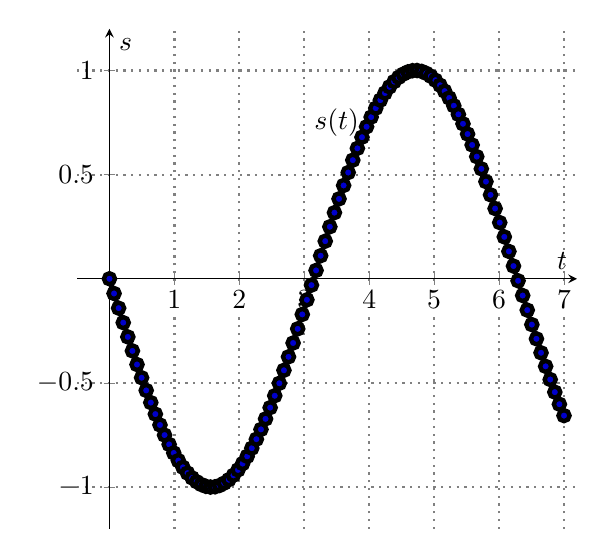
\begin{tikzpicture}
            \begin{axis}[axis x line=center, axis y line=middle,
            width=2.5in, height=2.5in, 
            scale only axis, %axis equal,
            xmin=-0.5, xmax=7.2,
            ymin=-1.2, ymax=1.2,
            xtick={0,...,7}, ytick={-1,-0.5,...,1},
            xticklabel style={draw=none, inner sep=2pt, fill=white, text opacity=1},
            xlabel={$t$}, ylabel={$s$},
            grid=both, grid style={line width=.8pt, draw=gray, dotted},
            minor tick num=0, 
            samples=100]
            \addplot+[black, ultra thick, domain=0:7] {-sin(x*180/pi)};
            \node at (3.5, 0.75) {$s(t)$};
            \end{axis}
            \end{tikzpicture}
            \tinysp
            
            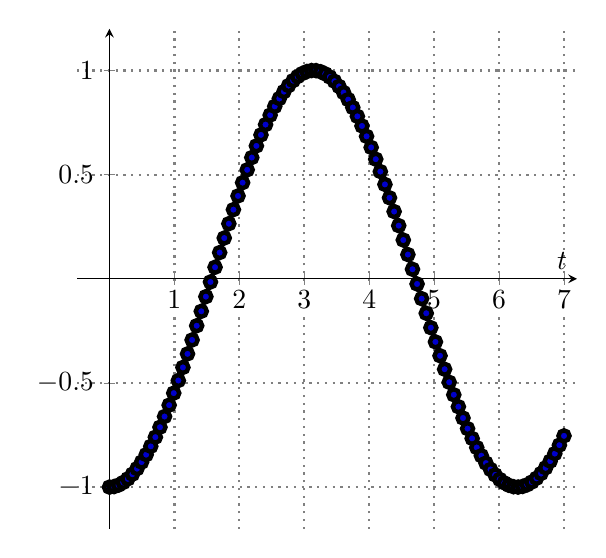
\begin{tikzpicture}
            \begin{axis}[axis x line=center, axis y line=middle,
            width=2.5in, height=2.5in, 
            scale only axis, %axis equal,
            xmin=-0.5, xmax=7.2,
            ymin=-1.2, ymax=1.2,
            xtick={0,...,7}, ytick={-1,-0.5,...,1},
            xticklabel style={draw=none, inner sep=2pt, fill=white, text opacity=1},
            xlabel={$t$}, ylabel={},
            grid=both, grid style={line width=.8pt, draw=gray, dotted},
            minor tick num=0, 
            samples=100]
            \addplot+[black, ultra thick, domain=0:7] {-cos(x*180/pi)};
            \end{axis}
            \end{tikzpicture}
            
            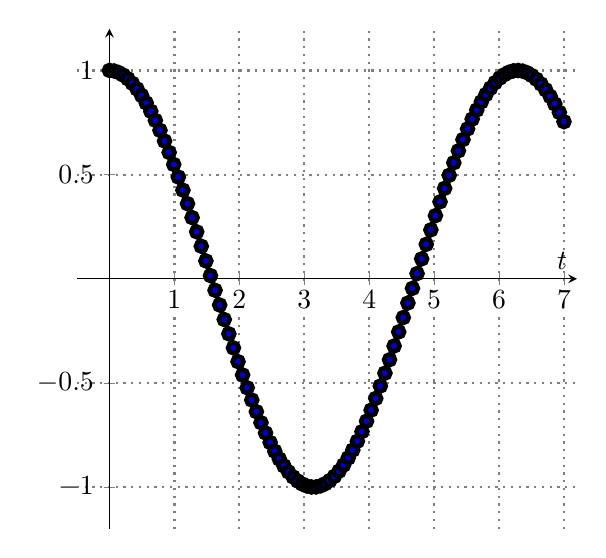
\begin{tikzpicture}
            \begin{axis}[axis x line=center, axis y line=middle,
            width=2.5in, height=2.5in, 
            scale only axis, %axis equal,
            xmin=-0.5, xmax=7.2,
            ymin=-1.2, ymax=1.2,
            xtick={0,...,7}, ytick={-1,-0.5,...,1},
            xticklabel style={draw=none, inner sep=2pt, fill=white, text opacity=1},
            xlabel={$t$}, ylabel={},
            grid=both, grid style={line width=.8pt, draw=gray, dotted},
            minor tick num=0, 
            samples=100]
            \addplot+[black, ultra thick, domain=0:7] {cos(x*180/pi)};
            \end{axis}
            \end{tikzpicture}
            \tinysp
            
            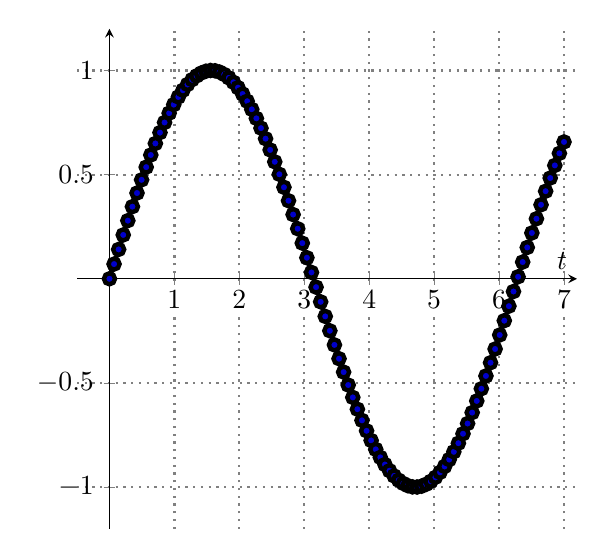
\begin{tikzpicture}
            \begin{axis}[axis x line=center, axis y line=middle,
            width=2.5in, height=2.5in, 
            scale only axis, %axis equal,
            xmin=-0.5, xmax=7.2,
            ymin=-1.2, ymax=1.2,
            xtick={0,...,7}, ytick={-1,-0.5,...,1},
            xticklabel style={draw=none, inner sep=2pt, fill=white, text opacity=1},
            xlabel={$t$}, ylabel={},
            grid=both, grid style={line width=.8pt, draw=gray, dotted},
            minor tick num=0, 
            samples=100]
            \addplot+[black, ultra thick, domain=0:7] {sin(x*180/pi)};
            \end{axis}
            \end{tikzpicture}
        \end{multicols}
    \end{multipartquestion}
\end{document}